
\documentclass[../main/SI3_manual]{subfiles}

\begin{document}
% ================================================================
% Chapter 1 � Model Basics
% ================================================================

\chapter{Model Basics}
\label{chap:MB}
\chaptertoc

\newpage
$\ $\newline    % force a new line

%-------------------------------------------------------------------------------------------------------------------------
%
% 2.1 Assumptions
\section{Rationale and assumptions}
%
%-------------------------------------------------------------------------------------------------------------------------
\begin{itemize}
\item Separation of horizontal dynamics and vertical thermodynamics;
\item Dynamics: sea ice is a viscous-plastic continuum;
\item Thermodynamics: sea ice is a mushy layer covered by snow
\item Subgrid-scale physics
\end{itemize}

\subsection{Scales, thermodynamics and dynamics}
Because sea ice is much wider -- $\mathcal{O}$(100-1000 km) -- than thick -- $\mathcal{O}$(1 m) -- ice drift can be considered as purely horizontal: vertical motions around the hydrostatic equilibrium position are negligible. The same scaling argument justifies the assumption that heat exchanges are purely vertical\footnote{The latter assumption is probably less valid, because the horizontal scales of temperature variations are $\mathcal{O}$(10-100 m)}. It is on this basis that thermodynamics and dynamics are separated and rely upon different frameworks and sets of hypotheses: thermodynamics use the ice thickness distribution \citep{thorndike_1975} and the mushy-layer \citep{worster_1992} frameworks, whereas dynamics assume continuum mechanics \citep[e.g.,][]{lepparanta_2011}. Thermodynamics and dynamics interact by two means: first, advection impacts state variables; second, the horizontal momentum equation depends, among other things, on the ice state.

\subsection{Subgrid scale variations}

Sea ice properties -- in particular ice thickness -- feature important changes at horizontal scales $\mathcal{O}$(1m) \citep{thorndike_1975}. An explicit representation of these variations is not and will not be -- at least in the next twenty years or so -- accessible to large-scale sea ice models. Yet important features, such as energy exchanges through the ice, quite non-linearly depend on ice thickness \citep{maykut_1986}; whereas ice motion depends on the presence of open water, thin and thick ice at the very least, suggesting that subgrid-scale variations in ice properties must be accounted for, at least in a statistical fashion \citep{maykut_1973}. 

%--------------------------------------------------------------------------------------------------------------------
%
% FIG x : Ice scheme
%
\begin{figure}[ht]
\begin{center}
\vspace{0cm}
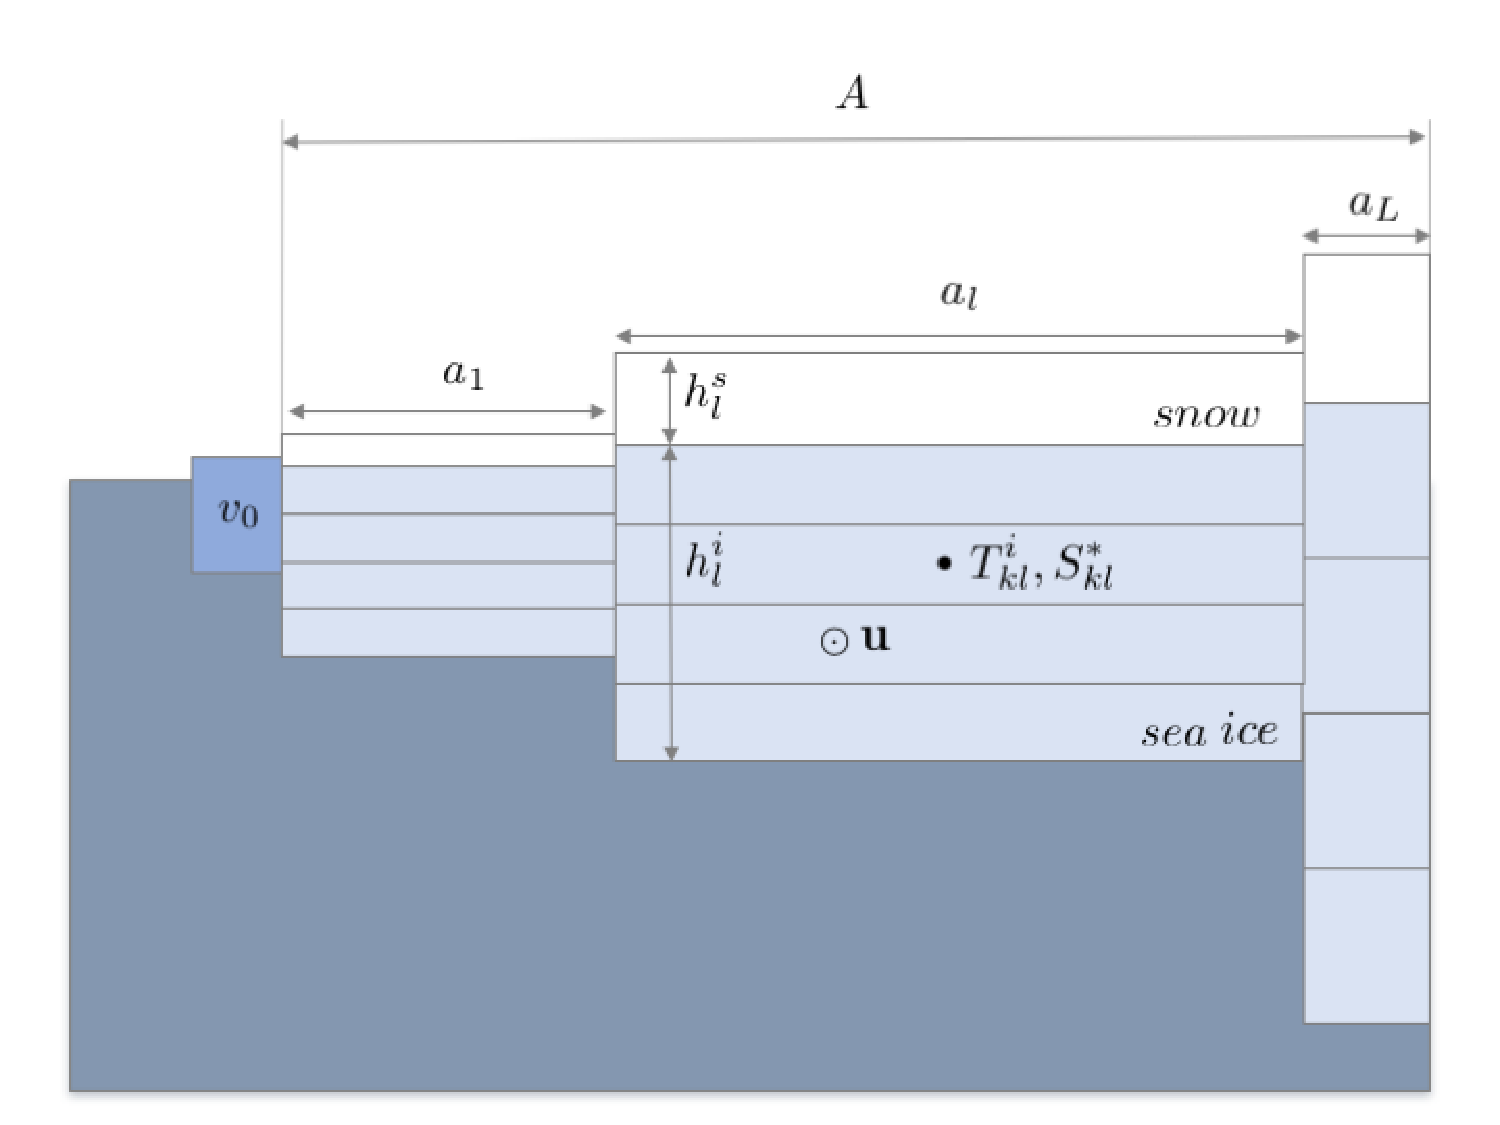
\includegraphics[height=10cm,angle=-00]{ice_scheme}
\caption{Representation of the ice pack, using multiple categories with specific ice concentration ($a_l, l=1, 2, ..., L$), thickness ($h^i_l$), snow depth ($h^s_l$), vertical temperature and salinity profiles ($T^i_{kl}$, $S^{*}_{kl}$) and a single ice velocity vector ($\mathbf{u}$).}
\label{ice_scheme}
\end{center}
\end{figure}
%
%--------------------------------------------------------------------------------------------------------------------

The \textit{multi-category} framework \citep{maykut_1973} addresses this issue by treating the ice thickness as an independent variable next to spatial coordinates and time, and introducing a thickness distribution\footnote{$g(h)$, termed the \textit{ice thickness distribution} is the density of probability of ice thickness \citep{thorndike_1975}.} $g(h)$ as the main prognostic model field. In the discrete world, the thickness distribution is converted into $L$ thickness categories. Ice thickness categories occupy a fraction of each grid cell, termed ice concentration ($a_l, l=1, 2, ..., L$), with specific thickness and properties. 

The \textit{single-category} framework \citep{hibler_1979} tackles the subgrid-scale issue by drastically simplifying the ice thickness distribution. The grid cell is divided into open water and sea ice characterized by a single ice concentration $A$ and mean thickness $H$. Single-category models (in particular LIM2) typically add parameterizations to represent the effects of unresolved ice thickness distribution on ice growth and melt \citep[see, e.g.][]{mellor_1989,fichefet_1997}.

SI$^3$ provides the choice between either a multi- or a single-category framework. The default mode is multi-category. The single-category mode can be activated by setting the number of categories ($jpl=1$) and by activating the virtual thickness distribution parameterizations (nn\_monocat=1).

\subsection{Thermodynamic formulation}

%
%--------------------------------------------------------------------------------------------------------------------
%
% TABLE x Physical constants
%
%
\begin{table}[ht]
\begin{footnotesize}
\caption{Thermodynamic constants of the model.}
\begin{center}
\begin{tabular}{@{}llccl}\hline
 & Description & Value & Units & Ref \\ \hline
$c_i$ (cpic) & Pure ice specific heat & 2067 & J/kg/K & ? \\
$c_w$ (rcp) & Seawater specific heat & 3991 & J/kg/K & \cite{teos-10_2010} \\
$L$ (lfus) & Latent heat of fusion (0$^\circ$C) & 334000 & J/kg/K & \cite{bitz_1999} \\
$\rho_i$ (rhoic) & Sea ice density & 917 & kg/m$^3$ & \cite{bitz_1999} \\
$\rho_s$ (rhosn) & Snow density & 330 & kg/m$^3$ & \cite{maykut_1971} \\
$\mu$ (tmut) & Linear liquidus coefficient & 0.054 & $^\circ$C/(g/kg) & \cite{assur_1958} \\
\hline
\end{tabular}
\end{center}
\label{PhysicalConstants_table}
\end{footnotesize}
\end{table}
%
%--------------------------------------------------------------------------------------------------------------------
%

Ice thermodynamics are formulated assuming that sea ice is covered by snow. Within each thickness category, both snow and sea ice are horizontally uniform, hence each thickness category has a specific ice thickness ($h_i^l$) and snow depth ($h_s^l$). Snow is assumed to be fresh, with constant density and thermal conductivity. Sea ice is assumed to be a \textit{mushy layer}\footnote{Mushy layers are two-phase, two-component porous media.} \citep{worster_1992} of constant density, made of pure ice and brine in thermal equilibrium, related by a linear liquidus relationship \citep{bitz_1999}. A vertically-averaged bulk salinity $S_l$ uniquely characterizes brine fraction for each thickness category, and changes through  time from a simple parametrization of brine drainage. The linear vertical salinity profile ($S^*_{kl}$) is reconstructed from the vertical mean \citep{vancoppenolle_2009}. The diffusion of heat affects the vertical temperature profile, discretized on a unique layer of snow and multiple ice layers (typically 2-5) for each category, whereas thermal properties depend on local brine fraction. Growth and melt rates are computed, also for each ice category. The choice of the main thermodynamic constants  is described in Tab. \ref{PhysicalConstants_table}.



%
%--------------------------------------------------------------------------------------------------------------------
%
% TABLE x Global variables
%
%
\begin{table}[ht]
\begin{footnotesize}
\caption{LIM global variables.}
\begin{center}
\begin{tabular}{@{}llcc}\hline
Symbol   & Description & Units & Code name \\ \hline
$\mathbf{u}$ & Sea ice velocity & [$m.s^{-1}$] & \textit{u\_ice, v\_ice (ji,jj)} \\
$\mathbf{\sigma}$ & Stress tensor & [$Pa.m$] & \textit{stress1\_i, stress2\_i} \\
 & & & \textit{stress12\_i (ji,jj)} \\
$a_l$ & Concentration of sea ice in category $l$ & [-] & \textit{a\_i(ji,jj,jl)} \\
$v^i_l$ & Volume of sea ice per unit area in category $l$ & [$m$] & \textit{v\_i(ji,jj,jl)} \\
$v^s_l$ & Volume of snow per unit area in category $l$ & [$m$] & \textit{v\_s(ji,jj,jl)} \\
$e^i_{kl}$ & Sea ice enthalpy per unit area in layer $k$ and category $l$ & [$J.m^{-2}$] & \textit{e\_i(ji,jj,jk,jl)} \\
$e^s_{l}$ & Snow enthalpy per unit area in category $l$ & [$J.m^{-2}$] & \textit{e\_s(ji,jj,jl)} \\
$M^s_l$ & Sea ice salt content in category $l$ & [$g/kg.m$] & \textit{smv\_i(ji,jj,jl)}\\
%$O_l$ & Sea ice age content in category $l$ & $[days.m]$ \\
\hline
\end{tabular}
\end{center}
\label{GVariables_table}
\end{footnotesize}
\end{table}
%
%--------------------------------------------------------------------------------------------------------------------

 Temperature, salinity, ice thickness, and snow depth are not extensive variables and therefore not conservative. Hence, conservative, extensive variables, must be introduced to ensure mass, salt and energy conservation. There are several back-and-forth conversions from extensive (conservative) state variables (see Table \ref{GVariables_table}) to intensive state variables of practical use (Table \ref{IVariables_table}).
 
 %--------------------------------------------------------------------------------------------------------------------
%
% TABLE x Equivalent variables
%
%
\begin{table}[ht]
\begin{footnotesize}
\caption{Intensive variables of practical use.}
\begin{center}
\begin{tabular}{@{}llcc}\hline
Symbol   & Description & Units \\ \hline
$h^i_l=v^i_l/g^i_l$ & Ice thickness & [$m$] \\
$h^s_l=v^s_l/g^i_l$ & Snow depth & [$m$] \\
$q^i_{m,kl}=e^i_{l,k}/(h^i_l/N)$ & Ice specific enthalpy & [$J.kg^{-1}$]\\
$q^s_{m,l}=e^s_{l}/h^s_l$ & Snow specific enthalpy & [$J.kg^{-1}$] \\
$T^i_{kl}=T(q^i_{kl})$ & Ice temperature & [$K$] \\
$T^s_{l} =T(q^s_{l}) $ & Snow temperature & [$K$] \\
$\overline S^i_{l}=M^s_l / v^i_l$ & Vertically-averaged bulk ice salinity & [g/kg] \\
$S^*_{kl}$ & Depth-dependent ice salinity & [g/kg] \\
$\phi_{kl}$ & Brine fraction & [-] \\
%$o^i_{l}=O_l / g^i_l $ & Ice age & [$days$] \\
\hline
\end{tabular}
\end{center}
\label{IVariables_table}
\end{footnotesize}
\end{table}
%
%--------------------------------------------------------------------------------------------------------------------

\subsection{Dynamic formulation}

The formulation of ice dynamics is based on the continuum approach. The latter holds provided the drift ice particles are much larger than single ice floes, and much smaller than typical gradient scales. This compromise is rarely achieved in practice \citep{lepparanta_2011}. Yet the continuum approach generates a convenient momentum equation for the horizontal ice velocity vector $\mathbf{u}=(u,v)$, which can be solved with classical numerical methods (here, finite differences on the NEMO C-grid). The most important term in the momentum equation is internal stress. We follow the viscous-plastic (VP) rheological framework \citep{hibler_1979}, assuming that sea ice has no tensile strength but responds to compressive and shear deformations in a plastic way. In practice, the elastic-viscous-plastic (EVP) technique of  \citep{bouillon_2013} is used, more convient numerically than VP.  It is well accepted that the VP rheology and its relatives are the minimum complexity to get reasonable ice drift patterns \citep{kreyscher_2000}, but fail at generating the observed deformation patterns \citep{girard_2009}. This is a long-lasting problem: what is the ideal rheological model for sea ice and how it should be applied are still being debated \citep[see, e.g.][]{weiss_2013}. 

%-------------------------------------------------------------------------------------------------------------------------
%
\section{Thickness distribution framework}
%
%-------------------------------------------------------------------------------------------------------------------------

We first present the essentials of the thickness distribution framework \citep{thorndike_1975}. Consider a given region of area $R$ centered at spatial coordinates $(\mathbf{x})$ at a given time $t$. $R$ could be e.g. a model grid cell. The ice thickness distribution $g(\mathbf{x},t, h)$ is introduced as follows:
\begin{linenomath}
\begin{align}
g(h) &= \lim_{dh \to 0} \frac{dA(h,h+dh)}{dh},
\end{align}
\end{linenomath}
where $dA(h,h+dh)$ is the surface fraction of all parts of $R$ with ice thickness between $h$ and $h+dh$. Using this definition, the spatial structure of ice thickness is lost (see Fig. \ref{fig_g_h}), and $h$ becomes an extra independent variable, next to spatial coordinates and time, that can be thought as random. $g$ is by definition normalized to 1. The conservation of area, expressed in terms of $g(h)$, is given by \citep{thorndike_1975}: 
\begin{linenomath}
\begin{align}
\frac{\partial g}{\partial t} = - \nabla .(g \mathbf{u}) - \frac{\partial}{\partial h} (f g) + \psi,
\label{eq:gt}
\end{align}
\end{linenomath}
where the terms on the right hand side refer to horizontal transport, thermodynamic transport in thickness space ($f$, m/s is the growth/melt rate), and mechanical redistribution rate, e.g. by ridging and rafting, where $\psi$ must conserve ice area and volume by construction.

%--------------------------------------------------------------------------------------------------------------------
%
% FIG x : Ice thickness distribution
%
\begin{figure}[ht]
\begin{center}
\vspace{0cm}
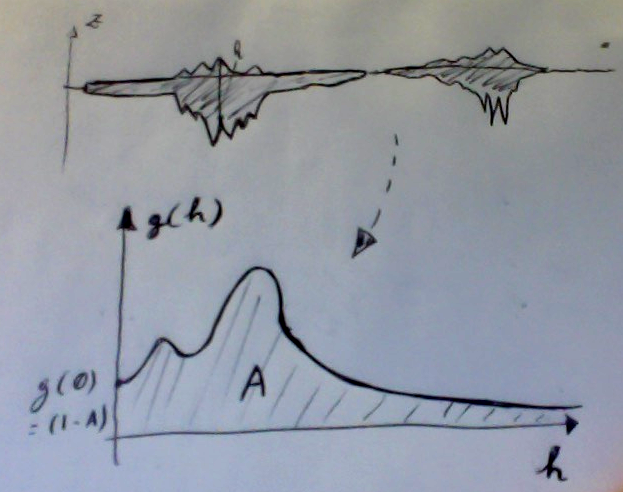
\includegraphics[height=6cm,angle=-00]{g_h}
\caption{Representation of the relation between real thickness profiles and the ice thickness distribution function $g(h)$}
\label{fig_g_h}
\end{center}
\end{figure}
%
%--------------------------------------------------------------------------------------------------------------------

In numerical implementations, the thickness distribution is discretized into several thickness categories, with specific ice concentration $a_l$ and ice volume per area $v_l^i$:
\begin{linenomath}
\begin{align}
a_l &= \int _{H^*_{l-1}}^{H^*_l} dh \cdot g(h) , \\
v_l^i &= \int _{H^*_{l-1}}^{H^*_l} dh \cdot h \cdot g(h).
\end{align}
\end{linenomath}
Ice volume per area is the extensive counterpart for ice thickness, connected with volume through $h_l^i = v_l^i / a_l$. Evolution equations for extensive variables can be readily derived from equation \ref{eq:gt} by integration between thickness boundaries of the $l^{th}$ category \citep{bitz_2001}. This applies to all model extensive variables (see Table \ref{GVariables_table}). For ice area, this reads:
\begin{linenomath}
\begin{align}
\frac{\partial a_l}{\partial t} = - \mathbf{\nabla} \cdot (a_l \mathbf{u}) + \Theta^a_l + \int_{H^*_{l-1}}^{H^*_l} dh \psi.
\label{eq:gt}
\end{align}
\end{linenomath}
wher $\Theta^a_l$ refers to the effect of thermodynamics. Enthalpy is a particular case because it also has a vertical depth dependence $z$, which corresponds to $K$ vertical layers of equal thickness. The solution adopted here, following from \cite{zhang_2001}, is that enthalpy from the individual layers are conserved separately. This is a practical solution, for lack of better.

One of the major actions of LIM is to resolve conservation equations for all extensive variables that characterize the ice state.  Let us now connect this detailed information with classical sea ice fields. The ice concentration $A$ and the ice volume per area\footnote{Ice volume per area is equivalent to the grid-cell averaged ice thickness.} $V_i$ (m) directly derive from $g$: 
\begin{linenomath}
\begin{align}
 A(\mathbf{x},t) &=\int_{0^+}^{\infty} dh \cdot g(h,\mathbf{x},t) \sim A_{ij} = \sum_{l=1}^L a_{ijl}, & \\
 V_i(\mathbf{x},t)&=\int_{0}^{\infty} dh \cdot g(h,\mathbf{x},t) \cdot h \sim V^i_{ij} = \sum_{l=1}^L v^i_{ijl}. & \\
\end{align}
\end{linenomath}
where the $0^+$ boundary implies that the means exclude open water. The mean ice thicknesses $H_i$ (m) is:
\begin{linenomath}
\begin{align}
H_i = V_i/A,
\end{align}
\end{linenomath}
whereas the open water fraction is simply $1-A$.

\section{Governing equations}

Let us now readily present the set of the LIM "governing" equations in the framework of the assumptions developed above. The conservation of horizontal momentum reads:
\begin{linenomath}
\begin{align}
m \frac{\partial \mathbf{u}} {\partial t} & = \mathbf{\nabla}\cdot\mathbf{\sigma} +A \left(\mathbf{\tau}_{a}+\mathbf{\tau}_{w}\right) - m f \mathbf{k} \times \mathbf{u} - m g \mathbf{\nabla}{\eta},
\label{a}
\end{align}
\end{linenomath}
where $m=\rho_i V_i + \rho_s V_s $ is the ice and snow mass per unit area, $\mathbf{u}$ is the ice velocity, $\mathbf{\sigma}$ is the internal stress tensor, $\mathbf{\tau}_a$ and $\mathbf{\tau}_w$ are the air and ocean stresses, respectively, $f$ is the Coriolis parameter, $\mathbf{k}$ is a unit vector pointing upwards, $g$ is the gravity acceleration and $\eta$ is the ocean surface elevation. The EVP approach used in LIM \citep{bouillon_2013} gives the stress tensor as a function of the strain rate tensor $\dot{\mathbf{\epsilon}}$ and some of the sea ice state variables:
\begin{linenomath}
\begin{align}
\mathbf{\sigma} & = \mathbf{\sigma} (\dot{ \mathbf{\epsilon}}, \text{ice state}).
\end{align}
\end{linenomath}
To the exception of velocity and internal stress, all extensive variables in Table \ref{GVariables_table} follow a conservation equation of the form:
\begin{linenomath}
\begin{align}
\frac{\partial X}{\partial t} & = - \nabla .(\mathbf{u}X) + \Theta^X + \Psi^X,
\label{eq:Xt}
\end{align}
\end{linenomath}
including the effets of transport, thermodynamics ($\Theta^X$) and mechanical redistribution ($\Psi^X$). Solving these $jpl.(4+2.jpk)$ equations gives the temporal evolution of $\mathbf{u}$, $\mathbf{\sigma}$ and the rest of the global (extensive) variables listed in Table \ref{GVariables_table}.

\section{Ice Dynamics}

Dynamical processes include the conservation of momentum, rheology, transport and mechanical redistribution.
To resolve the momentum equation, atmospheric stress is taken either as forcing or from an atmospheric model, oceanic stress and sea surface elevation from the ocean model, the Coriolis term is trivial. The last term, the divergence of the internal stress tensor $\sigma$, is the most critical term in the momentum equation and requires a rheological formulation. The EVP approach used in LIM gives the stress tensor components as \citep{bouillon_2013}:
\begin{linenomath}
\begin{align}
\sigma_{ij} & = \frac{P}{2(\Delta + \Delta_{min}) }
\biggr [ ( \dot{\epsilon}_{kk} - \Delta) \delta_{ij} + \frac{1}{e^2} ( 2 \dot{\epsilon}_{ij} - \dot{\epsilon}_{kk} \delta_{ij} ) \biggr ],
\end{align}
\end{linenomath}
where $\Delta$ is a particular measure of the deformation rate, $\Delta_{min}$ a parameter determining a smooth transition from pure viscous vlow ($\Delta<<\Delta_{min}$) to pure plastic flow ($\Delta >> \Delta_{min}$), and $e$ is a parameter giving the ratio between the maximum compressive stress and twice the maximum shear stress. In the pure plastic regime, the stress principal components should lie on the edge of an elliptical yield curve (Fig. \ref{fig_yield}). In the viscous regime, they are within the ellipse. The ice strength $P$ determines the plastic failure criterion and connects the momentum equation with the state of the sea ice. $P$ is not well constrained and must be parameterized. The heuristic option of \cite{hibler_1979} was here adopted as a reference formulation:
\begin{linenomath}
\begin{align}
P & = P^* V_i e^{-C(1-A)},
\end{align}
\end{linenomath}
where $P^*$ and $C$ are empirical constants (see Table \ref{Modelparameters_table} for the values of the main model parameters).

%--------------------------------------------------------------------------------------------------------------------
%
% FIG x : Ice thickness distribution
%
\begin{figure}[ht]
\begin{center}
\vspace{0cm}
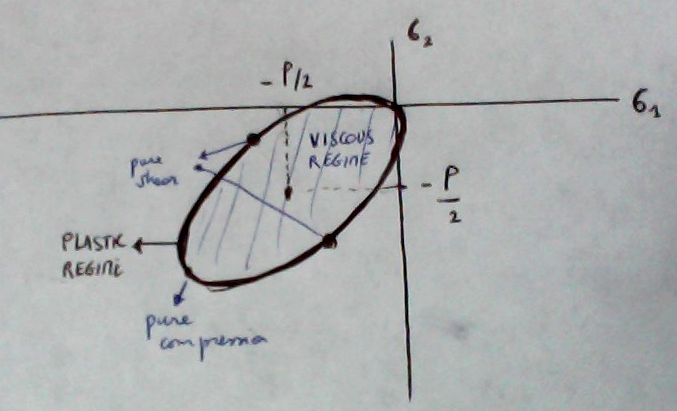
\includegraphics[height=6cm,angle=-00]{yield_curve}
\caption{Elliptical yield curve used in the VP rheologies, drawn in the space of the principal components of the stress tensor ($\sigma_1$ and $\sigma_2$).}
\label{fig_yield}
\end{center}
\end{figure}
%
%--------------------------------------------------------------------------------------------------------------------

%
%--------------------------------------------------------------------------------------------------------------------
%
% TABLE x Model parameters %
%
\begin{table}[ht]
\begin{footnotesize}
\caption{Main model parameters.}
\begin{center}
\begin{tabular}{@{}llccl}\hline
 & Description & Value & Units & Ref \\ \hline
 
% Parameters
$P*$ (rn\_pstar) & ice strength thickness param. & 20000 & N/m2 & - \\
$C$ (rn\_crhg) & ice strength concentration param. & 20 & - & \citep{hibler_1979} \\
$H^*$ (rn\_hstar) & maximum ridged ice thickness param. & 25 & m & \citep{lipscomb_2007} \\
$p$ (rn\_por\_rdg) & porosity of new ridges & 0.3 & - & \citep{lepparanta_1995} \\
$amax$ (rn\_amax) & maximum ice concentration & 0.999 & - & -\\
$h_0$ (rn\_hnewice) & thickness of newly formed ice & 0.1 & m & - \\
 
\hline
\end{tabular}
\end{center}
\label{Modelparameters_table}
\end{footnotesize}
\end{table}
%
%--------------------------------------------------------------------------------------------------------------------
%


Transport connects the horizontal velocity fields and the rest of the ice properties. LIM assumes that the ice properties in the different thickness categories are transported at the same velocity. The scheme of \cite{prather_1986}, based on the conservation of 0, 1$^{st}$ and 2$^{nd}$ order moments in $x-$ and $y-$directions,  is used, with some numerical diffusion if desired. Whereas this scheme is accurate, nearly conservative, it is also quite expensive since, for each advected field, five moments need to be advected, which proves CPU consuming, in particular when multiple categories are used. Other solutions are currently explored.

The dissipation of energy associated with plastic failure under convergence and shear is accomplished by rafting (overriding of two ice plates) and ridging (breaking of an ice plate and subsequent piling of the broken ice blocks into pressure ridges). Thin ice preferentially rafts whereas thick ice preferentially ridges \citep{tuhkuri_2002}. Because observations of these processes are limited, their representation in LIM is rather heuristic. The amount of ice that rafts/ridges depends on the strain rate tensor invariants (shear and divergence) as in \citep{flato_1995}, while the ice categories involved are determined by a participation function favouring thin ice \citep{lipscomb_2007}. The thickness of ice being deformed ($h'$) determines whether ice rafts ($h'<$ 0.75 m) or ridges ($h'>$ 0.75 m), following \cite{haapala_2000}. The deformed ice thickness is $2h'$ after rafting, and is distributed between $2h'$ and $2 \sqrt{H^*h'}$ after ridging, where $H^* = 25$ m \citep{lipscomb_2007}. Newly ridged ice is highly porous, effectively trapping seawater. To represent this, a prescribed volume fraction (30\%) of newly ridged ice \citep{lepparanta_1995} incorporates mass, salt and heat are extracted from the ocean. Hence, in contrast with other models, the net thermodynamic ice production during convergence is not zero in LIM, since mass is added to sea ice during ridging. Consequently, simulated new ridges have high temperature and salinity as observed \citep{hoyland_2002}. A fraction of snow (50 \%) falls into the ocean during deformation.

\section{Ice thermodynamics}
In this section, we develop the underlying principles of the thermodynamic formulation, summarized in the term $\Theta^X$, where $X$ refers to all extensive state variables. $\Theta^X$ includes the contributions of transport in thickness space and thermodynamic source and sink terms.

\subsection{Transport in thickness space}
Transport in thickness space describes how vertical growth and melt moves ice state variables among the different thicknesses at a velocity $f(h)$, the net ice growth/melt rate, which needs to be first computed.  In discretized form, this term moves ice properties between neighbouring categories. The linear remapping scheme of \cite{lipscomb_2001} is used. This scheme is semi-lagrangian, second-order, is less diffusive and converges faster than other options.

\subsection{Thermodynamic source and sink terms}

Since heat, salt and mass are strongly inter-dependent for sea ice, the thermodynamic source and sink terms are treated together. They include the changes in extensive sea ice state associated with thermodynamic processes. The latter are separated in two main parts: (i) open water fraction processes, where atmosphere and ocean are in direct interaction; and (ii) vertical ice thermodynamic processes, driven by surface snow/ice-atmosphere and basal ice-ocean exchanges, for each thickness category. For each part, first, the energy available or lost is specified. Then the impact on mass exchanges is evaluated. The latter part requires to specify how sea ice and snow responds to energy supply or loss, which is achieved through the enthalpy formulation.

%\subsubsection{Atmosphere-ice-ocean heat and mass exchanges}
%
%The atmosphere-ice heat exchanges are either specified in external files (forcing) or computed from an atmospheric model. The following heat and mass fluxes should be specified:
%\begin{itemize}
%\item Net solar flux, for open water ($Q^{sol}$) and ice categories ($Q^{sol,ice}_{l}$);
%\item Net non-solar flux, for open water ($Q^{nsol}$) and ice categories ($Q^{nsol,ice}_{l}$);
%\item Solid and liquid precipitation (kg/m$^2$/s).
%\end{itemize}
%
%In terms of mass (freshwater), the ocean gets:
%\begin{itemize}
%\item All liquid precipitation;
%\item The part of solid precipitation that is not intercepted by the ice, accounting for the part that is blown off the sea ice by winds;
%\item The net melting minus freezing mass flux, as diagnosed from thermodynamic sea ice calculations.
%\end{itemize}
%
%In terms of energy, the ocean gets:
%\begin{itemize}
%\item The net atmospheric solar flux, minus what is intercepted by the ice; plus what is transmitted below the ice; 
%\item The net atmospheric non-solar heat flux, minus what is used by the sea ice; 
%\item The sensible heat exchange associated with ice-ocean and atmosphere-ocean mass fluxes. 
%\end{itemize}
%
%In terms of salt, the ocean gets the net salt release minus uptake associated with sea ice growth, melt and brine drainage. There is no atmosphere-ocean salt flux.

\subsubsection{Enthalpy formulation}

% Add snow and water

A first overarching aspect of the thermodynamic calculations is the specification of the response of sea ice to energy supply. This is achieved by defining the internal energy (or enthalpy\footnote{Wording it internal energy or enthalpy is equivalent since pressure effects are not considered.}). This ultimately relies on the response of the phase composition to salinity and temperature changes. The enthalpy formulation used in LIM is based on the following assumptions:
\begin{itemize}
\item Sea ice is gas-free, composed solely of pure ice and saline brine, characterized by brine fraction $\phi$;
\item brine and pure ice are in thermodynamic equilibrium;
\item the salinity-dependence of the freezing point is linear (linear liquidus);
\item the density of the sea ice (ice+brine) medium is constant ($\rho_i$).
\end{itemize}
%In this context, the bulk salinity of a small control sea ice volume is related to the salinity of brine ($S_{br}$):
%\begin{linenomath}
%\begin{align}
%S = \phi S_{br}
%\label{eq_S_Sbr}
%\end{align}
%\end{linenomath}
%Because of thermal equilibrium and linear liquidus, brine salinity directly depends on local temperature: $T=-\mu S_{br}$. Hence, brine fraction is given by
%\begin{linenomath}
%\begin{align}
%\phi = -\frac{\mu S}{T}.
%\end{align}
%\end{linenomath}
%This equation relates brine fraction to bulk salinity and temperature, which therefore can be seen as the two main state variables in this linear mushy layer formulation for sea ice thermodynamics. 

%--------------------------------------------------------------------------------------------------------------------
%
% FIG x : Thermal properties
%
\begin{figure}[ht]
\begin{center}
\vspace{0cm}
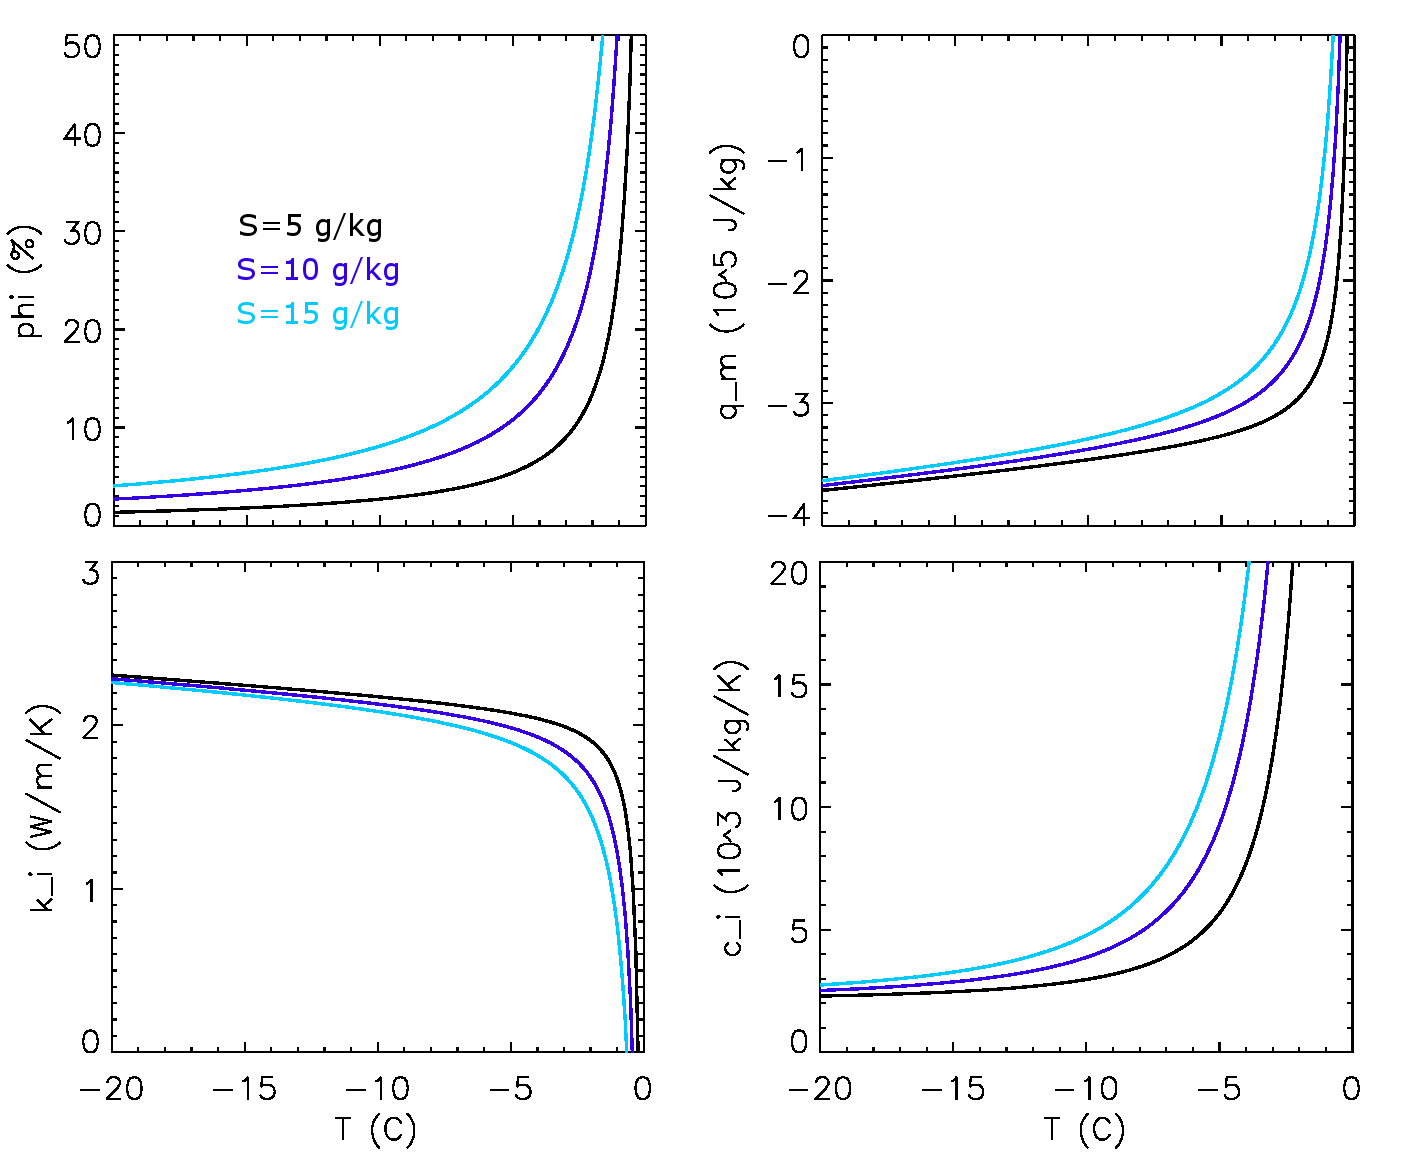
\includegraphics[height=8cm,angle=-00]{Thermal_properties}
\caption{Thermal properties of sea ice vs temperature for different bulk salinities: brine fraction, specific enthalpy, thermal conductivity, and effective specific heat.}
\label{fig_thermal_properties}
\end{center}
\end{figure}
%
%--------------------------------------------------------------------------------------------------------------------

Based on these, brine fraction reduces to $\phi = -\mu S/T$ (see Fig. \ref{fig_thermal_properties}), where $\mu$ relates the freezing point of brine to salinity, and one can derive the specific enthalpy $q_m(S,T)$, defined as the energy required to warm and melt a unit control volume of sea ice at temperature $T$ (in Celsius) and salinity $S$ until 0$^\circ$ C, taken as a reference zero-energy level \citep{bitz_1999,schmidt_2004}:
\begin{linenomath}
\begin{align}
q_m(S,T) = \biggr [ c_i ( T + \mu S) - L \biggr ( 1 + \frac{\mu S}{T} \biggr ) - c_w \mu S \biggr ]
\end{align}
\end{linenomath}
where $c_i$ is pure ice specific heat, $L$ is latent heat of fusion at 0$^\circ$C, and $c_w$ is water specific heat. The first term expresses the warming of solid ice. The second term expresses internal change in brine fraction, which is often the largest because the Stefan number  ($c_i T/L$) is generally small. The last term gives the warming of the remaining water from $T_{fr} = -\mu S$ until 0$^\circ$C. Similar, but simpler and linear expressions for snow and water can be derived.

The second overarching aspect is that all growth and melt processes must be calculated consistently with the enthalpy formulation. Energetics of phase transitions are handled using the formalism of \cite{schmidt_2004}. For each phase transition, initial and final states (temperature and salinity) are defined, and the ice-to-ocean mass flux to the ice $F_m$ (kg/s) relates to the energy gain or loss $\Delta Q$ through:
\begin{linenomath}
\begin{align}
\Delta Q / \Delta q_m = F_m,
\label{eq_phasechange}
\end{align}
\end{linenomath}
where $\Delta q_m$ is the change in specific enthalpy involved in the considered phase transition, from initial to final state.


\subsubsection{Open water processes}

As part of the sea ice thermodynamic calculations, a heat budget estimate for the uppermost ocean level ($B^{opw}$) must be included, to compute the rate of new ice formation or the contribution of sensible heat to bottom melting. $B^{opw}$ includes:
\begin{itemize}
\item the absorption of a fraction $f_1^{qsr}$ of solar radiation (given by radiative transfer component of the ocean model);
\item the non-solar heat flux absorbed at the surface;
\item the sensible heat content of precipitation
\item the sensible heat flux from the ocean to the sea ice ($A.F_w$)
\end{itemize}
Other contributions are not assumed not to contribute. The ocean-to-ice sensible heat flux is formulated the bulk formula of \citep{mcphee_1992}.

% Ice growth
If $B^{opw}$ is such that the SST would decrease below the freezing point, the remainder of the heat is used to form new ice. The heat loss is converted into a volume of new ice $v_0$. The thickness $h_0$ of the new ice grown during a sea ice time step depends on unresolved small-scale currents and waves and is prescribed. The fraction $a_0=v_0/h_0$ is computed accordingly. The salinity of this new ice $S_0$ is given by the salinity-thickness empirical relationship of \cite{kovacs_1996}. The temperature assumed for this new ice is the local freezing point. If by contrast $B^{opw}$ is positive and there still is ice in the grid cell, then $B^{opw}$ is directly redirected to bottom melting. This argument follows from \cite{maykut_1995}, who found that most of solar heat absorbed in the surface waters is converted into melting. In practise, this prevents the SST to be above freezing as long ice is present.

$B^{opw}$ can be seen as a predictor of the heat budget of the first ocean level. As such, it only helps to compute new ice formation and the extra bottom melt in summer, but is not part of the conservation of heat in the model. To ensure heat conservation, the heat effectively contributing to changing sea ice is removed from the non-solar flux sent to the ocean. This includes: (i) the heat loss used for ice formation, (ii) the heat gain used to melt ice, and (iii) the sensible heat given by the ocean to the ice. Finally, because ice dynamics are not able to maintain the small amount of open water that is observed, a maximum ice fraction ($amax, <1$) is prescribed.

\subsubsection{Vertical ice thermodynamic processes}

The second part of the computations regard the computation of purerly vertical processes in the ice-covered part of the grid cell, similarly for each ice category. 

\textbf{Surface melt, basal growth and melt and diffusion of heat}. The surface melt rate, as well as the basal growth / melt rate depend on the energy budget at the upper and lower interfaces, respectively, between the external fluxes either from the atmosphere or the ocean, and the internal conduction fluxes. The internal conduction fluxes depend on the internal temperature profile, which is determined by solving the enthalpy equation:
\begin{linenomath}
\begin{align}
\rho \frac{\partial q_m}{\partial t} = - \frac{\partial}{\partial z} (F_c + F_r ).
\end{align}
\end{linenomath}
which state that the local change in enthalpy is given by the divergence of the vertical conduction ($F_c=-k(S,T) \partial T / \partial z$) and radiation ($F_r$) fluxes. $\rho$ is the density of ice or snow. Re-expressed as a function of temperature, this becomes the heat diffusion equation.  This equation is non-linear in $T$, because of $q$ and $k$, and its main specificity is that internal melting requires large amounts of energy near the freezing point. The thermal conductivity is formulated following \cite{pringle_2007}, empirically accounting for the reduction of thermal conductivity at large brine fractions. 

At the ice base, we assume that the temperature is at the local freezing point.  Ice grows or melt if the heat balance between the oceanic sensible heat flux ($F_w$) and internal conduction is negative or positive.

At the ice surface, the boundary condition on the heat diffusion equation is:
\begin{linenomath}
\begin{align}
Q^{sr}  + Q^{ns}(T_{su})= F_c + Q^{sum}.
\end{align}
\end{linenomath}
where $Q^{sr}$ and $Q^{ns}$ are the net downwelling atmospheric solar and non-solar flux components. If the solution of this equation without melting gives a surface temperature ($T_{su}$) below 0$^\circ$ C, then there is no melting and the heat available for surface melting $Q_{sum}=0$.  Otherwise $T_{su}$ is capped at 0$^\circ$ C and $Q_{sum}$ is calculated as a residual.

\textbf{Radiation}. Radiation contributes to the surface and internal heat budget. The radiative transfer scheme is currently basic, composed of surface albedo, transmission through the ice interior and attenuation with vertical depth. The albedo is computed empirically as a function of ice thickness, snow depth and surface temperature, using a reformulation of the parameterization of \cite{shine_1985}. When snow is present, all the absorbed radiation is transformed into sensible heat available for conduction or melting. Over snow-free ice, a fraction of solar radiation is transmitted below the surface and attenuates exponentially with depth, until it reaches the base of the ice.

\textbf{Growth and melt processes}.  Snow grows from precipitation and loses mass from melting and snow-ice conversion once the snow base is below sea level. Sea ice grows and melts by various means. Ice forms by congelation or melt at the base, can melt at the surface and form from snow-to-ice conversion at the snow-ice interface if the latter is below sea level. Some new ice is also added to the system when seawater is trapped into newly formed pressure ridges.

\textbf{Salt dynamics}. Bulk salinity is empirically parameterized, as a function of salt uptake during growth, gravity drainage and flushing. The shape of the vertical profile depends on the bulk salinity \citep{vancoppenolle_2009}.

\textbf{Single-category parameterizations}. If the single-category representation is adopted, then two parameterizations can be activated, following \citep{fichefet_1997}. First, the thermal conductivity of both ice and snow is multiplied by a factor $>1$ accounting for the unresolved thin ice, effectively increasing the ice growth rate. Second, to account for the loss of thin ice in summer, the ice concentration is reduced in proportion to the loss of ice thickness. Both parameterizations have been tuned to match the results in multi-category mode.

\end{document}